\subsection{DHCP and static IP}
To analyse the power consumption when connecting via DHCP or with a static IP, we monitored the current of an average connection process.\\

\subsubsection{Experimental setup}
The sequence of the test program for DHCP is the same as Fig. \ref{fig:experiment_deep_sleep} shows.
Fig. \ref{fig:experiment_static_ip} shows the sequence when conducting the experiment using a static IP address.
The ESP8266WiFi library provides functionality to set a fixed IP address for our device.\\

\subsubsection{DHCP}
As shown you can see in Fig. \ref{fig:dhcp}, the connection to the WiFi network by using DHCP takes approximately 5.5 seconds and there are three spikes where the ESP8266 takes 140-120 milliamps.
In average, the energy consumption is about 68.9 milliamps.

\begin{figure}[h]
    \centering
    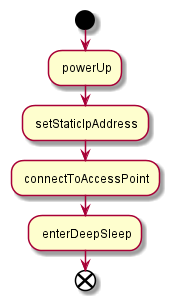
\includegraphics[width = 0.35 \linewidth]{fig/sequence_static_ip.png}
    \caption{Experimental setup for use of a static IP.}
    \label{fig:experiment_static_ip}
\end{figure}
\begin{figure}[h]
    \centering
    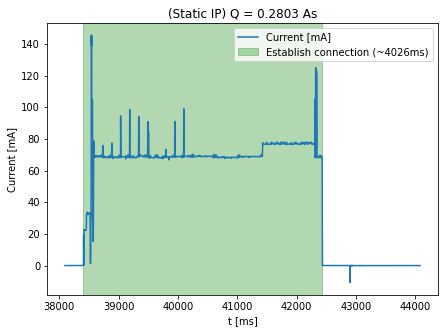
\includegraphics[width =\linewidth]{fig/static_ip.png}
    \caption{Experimental setup for use of a static IP.}
    \label{fig:static_ip}
\end{figure}
\begin{figure}[h]
    \centering
    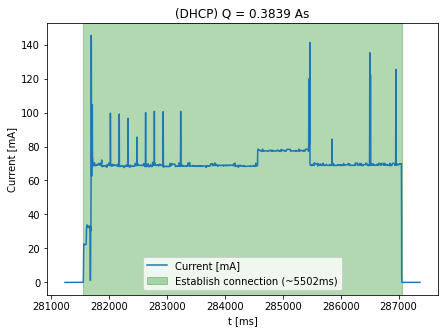
\includegraphics[width =\linewidth]{fig/dhcp.png}
    \caption{Experimental setup for use of a static IP.}
    \label{fig:dhcp}
\end{figure}